\chapter{Superposition}

\section{Principle of Superposition}

\begin{principle}[Principle of Superposition]
    When two or more waves of the same type meet, the resultant displacement is the vector sum of the individual displacements of the waves.
\end{principle}

\begin{definition}
    When the phase difference between two waves at a point is an integer multiple of a cycle ($\D \f = 2k\pi$), the waves are in \vocab{phase}. When the phase difference is an odd integer multiple of a half cycle ($\D \f = (2k + 1)\pi$), the waves are in \vocab{anti-phase}.
\end{definition}

\begin{definition}
    \vocab{Interference} is the result of superposing two or more waves of the same type.
\end{definition}

In particular, when two waves of the same frequency and amplitude superpose in phase, they reinforce each other and the resultant displacement is twice that of each individual wave. This is called \vocab{constructive interference}.

In contract, when two waves of the same frequency and amplitude superpose in anti-phase, they cancel each other and the resultant displacement is zero. This is called \vocab{destructive interference}.

A result between the two extremes is called a \vocab{partial interference}.

\begin{definition}
    Two waves of the same type and frequency are said to be \vocab{coherent} if there is a constant phase difference between them.
\end{definition}

Two wave sources are said to be coherent if the waves they produce are coherent.

\begin{definition}
    The \vocab{path difference} to a particular point from two wave sources is the difference in path lengths from the two sources to that point.
\end{definition}

\section{Stationary Waves}

\begin{definition}
    A wave is said to be \vocab{stationary} (or \vocab{standing}) if energy is not transferred, but stored in the oscillations of the medium.
\end{definition}

When two progressive waves of the same type of equal amplitude, equal frequency, and equal speed travelling in opposite directions meet, the resultant wave is stationary.

\begin{definition}
    A \vocab{node} is a point on a standing wave where the displacement is always zero.
\end{definition}

\begin{definition}
    An \vocab{anti-node} is a point on a standing wave with maximum amplitude.
\end{definition}

\begin{figure}[H]
    \centering
    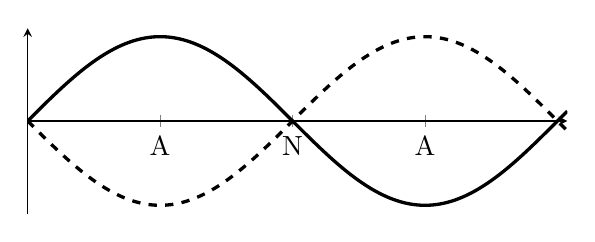
\begin{tikzpicture}[trim axis left, trim axis right]
        \begin{axis}[
            domain=0:6.4,
            xmax = 6.4,
            xmin = 0,
            ymin = -1.1,
            ymax = 1.1,
            axis equal image,
            axis y line=middle,
            axis x line=middle,
            samples=200,
            xtick = {pi/2, pi, 3*pi/2},
            xticklabels = {A , N, A},
            ytick = \empty,
            xlabel = \empty,
            ylabel = \empty,
            legend cell align={left},
            legend pos=outer north east,
            ]
            
            \addplot[black, very thick] {sin(deg(x))};

            \addplot[black, dashed, very thick] {-sin(deg(x))};
        \end{axis}
    \end{tikzpicture}
    \caption{Nodes and anti-nodes on a standing wave.}
\end{figure}

Nodes occur when the two underlying progressive waves meet in anti-phase, while anti-nodes occur when the two underlying progressive waves meet in phase.

The distance between two adjacent nodes or two adjacent anti-nodes is $\l/2$, where $\l$ is the wavelength of the underlying progressive waves as well as that of the resultant stationary wave.

In a stationary wave, all particles within a loop vibrate in phase, but have a phase difference of $\pi$ rad with particles in an adjacent loop.

\subsection{Stationary Waves in Stretched Strings}

\begin{figure}[H]
    \centering
    \includegraphics[scale=0.4]{media/Stationary Wave in Stretched String.png}
    \caption{Generating stationary waves in a stretched string.\protect\footnotemark}
\end{figure}
\footnotetext{Source: \url{https://physicslabs.ccnysites.cuny.edu/labs/208/208-vibrating-strings/vibrating-strings.php}}

The set up above shows how stationary waves can be produced in strings.

A string of length $L$ is held taut by connecting a mass on one end through a pulley and the other end to an oscillator. A frequency generator is used to vary the frequency of the oscillation.

The progressive wave produced by the oscillator moves towards the pulley with a constant velocity $v$. The wave is reflected at the pulley and travels backwards. The incident and reflected waves have the same speed, frequency and amplitude, moving in opposite directions.

For a stationary wave to form, the wave must have a node at both ends of the string. That is, there must be an integer number of loops on the length of the string. The resultant stationary wave is known as a \vocab{harmonic}.

\begin{proposition}
    In a string, the $n$th harmonic occurs when $n$ loops fit exactly into the length of the string. \[L = n\bp{\frac{\l}{2}} \quad \text{for $n = 1, 2, 3, \dots$}.\]
\end{proposition}

\begin{figure}[H]
    \centering
    \includegraphics[scale=0.4]{media/Harmonics in a String.png}
    \caption{The first four harmonics ($n = 1, 2, 3, 4$).\protect\footnotemark}
\end{figure}
\footnotetext{Source: \url{https://standingwavesch4.wordpress.com/harmonics/}}

\subsection{Stationary Waves in Air Columns}

Stationary waves can be formed in both closed pipes (open at only one end) and open pipes (open at both ends).

When air is blown into the open end of the pipe, a wave travels from the open end towards the closed end. The wave is reflected when it hits the wall of the closed end of the pipe. A stationary wave forms only if the closed ends are nodes and the open ends are anti-nodes.

\begin{figure}[H]
    \centering
    \includegraphics[scale=0.7]{media/Harmonics in a Pipe.png}
    \caption{The first four harmonics in an open and closed pipe.\protect\footnotemark}
\end{figure}
\footnotetext{Source: \url{https://link.springer.com/article/10.1007/s00233-019-10059-4}}

In practice, the anti-node at the open end occurs slightly outside the pipe. Hence, there is an \vocab{end correction} ($c$) that needs to be considered when calculating the wavelength or frequency of the wave.

\begin{proposition}
    In an open pipe, the $n$th harmonic occurs when $n$ A-N-A cycles fit exactly into the length of the pipe (accounting for end corrections). \[L = n \bp{\frac{\l}{2}} + 2c \quad \text{for $n = 1, 2, 3, \dots$}.\]
\end{proposition}

\begin{proposition}
    In a closed pipe, the $n$th harmonic occurs when $n$ A-N-A cycles fit exactly into \emph{twice} the length of the pipe (accounting for end corrections).\[2L = n \bp{\frac\l2} + 2c \quad \text{for $n = 1, 3, 5, \dots$}.\]
\end{proposition}

Note that closed pipes only have odd harmonics.

\section{Diffraction}

When waves encounter an obstacle or an opening, they will spread out after passing through an opening or around the edge of the obstacle.

\begin{definition}
    \vocab{Diffraction} is the spreading of a wave as it passes through a gap or around an obstacle.
\end{definition}

The spreading of the wavefronts becomes more pronounced when the size of the slit or \vocab{aperture} ($a$) is of the same order as the wavelength ($\l$), i.e. $a \approxeq \l$. However, it is negligible when the width is large in comparison to the wavelength, i.e. $a \gg \l$.

\begin{figure}[H]
    \centering
    \includegraphics[scale=0.4]{media/Apeture.jpg}
    \caption{The significance of the spreading depends on the relative size of the aperture.\protect\footnotemark}
\end{figure}
\footnotetext{Source: \url{https://www.alamy.com/wave-diffraction-wave-impinges-on-a-narrow-and-a-broad-slit-comparison-of-large-and-small-opening-waves-spread-out-beyond-the-gap-vector-diagram-image473787292.html}}

\subsection{Single Slit Diffraction}

The figure below shows the experimental arrangement for observing the diffraction of light through a narrow slit of width $b$. A viewing screen is placed at a distance $L$ ($\gg b$) behind the slit.

\begin{figure}[H]
    \centering
    \begin{tikzpicture}[scale=0.6]
        \draw (-0.1, 3) rectangle (0.1, 0.5);
        \draw (-0.1, -3) rectangle (0.1, -0.5);

        \draw (7.4, 3) rectangle (7.6, -3);

        \draw[->-=0.5] (-3, 0) -- (-0.3, 0);
        \draw[->-=0.5] (-3, 1) -- (-0.3, 1);
        \draw[->-=0.5] (-3, 2) -- (-0.3, 2);
        \draw[->-=0.5] (-3, -1) -- (-0.3, -1);
        \draw[->-=0.5] (-3, -2) -- (-0.3, -2);

        \draw[dashed] (0.3, 0) -- (7.2, 0);
        \node[anchor=north] at (3.75, 0) {$L$};

        \draw (0.3, 0.5) -- (0.7, 0.5);
        \draw (0.3, -0.5) -- (0.7, -0.5);

        \draw[->] (0.5, 1) -- (0.5, 0.5);
        \draw[->] (0.5, -1) -- (0.5, -0.5);
        \node[anchor=south] at (0.5, 1) {$b$};
    \end{tikzpicture}
    \caption{The set-up for a single slit experiment.}
\end{figure}

The light pattern on the screen consists of a central maximum flanked by a series of weaker secondary maxima and dark fringes. It is also observed that the central maximum is significantly broader and brighter than the secondary maxima.

\begin{proposition}
    Points of zero intensity (i.e. dark fringes) occur at angles $\t$ satisfying \[b \sin \t = m \l \quad \text{for $m = \pm 1, \pm 2, \pm 3, \dots$}.\]
\end{proposition}

\begin{figure}[H]
    \centering
    \begin{tikzpicture}[trim axis left, trim axis right]
        \begin{axis}[
            domain = -3:3,
            xmin = -3,
            xmax = 3,
            ymin = 0,
            ymax = 3,
            axis equal image,
            samples = 200,
            axis y line=middle,
            axis x line=middle,
            xtick = {0, 0.8975, -0.8975, 1.7952, -1.7952, 2.6928, -2.6928},
            xticklabels = {0, $\frac{\l}{b}$, $-\frac{\l}{b}$, $\frac{2\l}{b}$, $-\frac{2\l}{b}$, $\frac{3\l}{b}$, $-\frac{3\l}{b}$},
            ytick = \empty,
            xlabel = {$\sin \t$},
            ylabel = {$I$},
            legend cell align={left},
            legend pos=outer north east,
                    after end axis/.code={
            \path (axis cs:0,0) 
                node [anchor=north] {$O$};
            }
            ]

            \addplot[very thick, red] {2.5 * (sin(3.5*deg(x))/(3.5*x))^2};            
        \end{axis}
    \end{tikzpicture}
    \caption{The intensity distribution for a single slit diffraction.}
\end{figure}

\subsection{Rayleigh's Criterion}

The \vocab{resolving power} of an optical instrument refers to its ability to distinguish between the images of relatively close objects.

Resolving power is often limited by diffraction phenomenon. The images from two separate points cannot be distinguished if the central maxima of their diffraction pattern overlaps. They are considered to be \vocab{just resolved} if the central maxima of their images coincides with the first minima of the other.

\begin{proposition}[Rayleigh Criterion]
    For the two points to be just resolved, the central maximum of one must lie on the first minimum of the other, i.e. \[b \sin \t = \l,\] where $\t$ is the angle between the two sources.
\end{proposition}

\begin{figure}[H]
    \centering
    \includegraphics[scale=1]{media/Rayleigh's Criterion.png}
    \caption{A sketch of Rayleigh's criterion.\protect\footnotemark}
\end{figure}
\footnotetext{Source: \url{https://xmphysics.com/2023/01/02/10-5-5-rayleighs-criterion-2/}}

\section{Two-Source Interference}

A stationary wave is an example of two-source interference of waves travelling in opposite directions. The nodes and anti-nodes are examples of destructive and constructive interference respectively.

\subsection{Water Waves}

When two dippers are attached to the oscillator of a ripple tank, two sets of circular water waves are generated and superpose. The resulting interference pattern is shown below.

\begin{figure}[H]
    \centering
    \includegraphics[scale=0.2]{media/Water Wave Interference Pattern.jpg}
    \caption{Interference pattern produced by water waves.\protect\footnotemark}
\end{figure}
\footnotetext{Source: \url{https://www.youtube.com/watch?v=fjaPGkOX-wo}}

Note that the two dippers are coherent sources since they are attached to the same oscillator.

Constructive interference occurs at points where the waves meet in phase (i.e. the path differences from the two sources are an integer number of wavelengths). These points form lines called \vocab{anti-nodal lines}.

Destructive interference occurs at points where the waves meet in anti-phase (i.e. the path differences are a half-integer number of wavelengths). These points form lines called \vocab{nodal lines}.

\subsection{Observable Interference}

Conditions for interference patterns to be observable, besides the obvious condition that the waves must superpose, include the following:
\begin{itemize}
    \item The waves must be coherent. For light waves, this condition implies that they must be monochromatic.
    \item The waves must have the same amplitude.
    \item For transverse waves, they must be either unpolarized or polarized in the same plane.
\end{itemize}

Note that two separate light sources are not coherent.

\subsection{Young's Double-Slit Experiment}

A \vocab{Young's double-slit experiment} involves passing light from a monochromatic source through a single slit followed by a double slit, as shown in the following diagram.

Diffraction at the single slit produces a point light source. Diffraction at the double slits produces two coherent light sources.

The lights from the double splits superpose on the screen with alternate constructive and destructive interference, resulting in a fringe pattern of bright and dark lines on the screen.

The bright lines on the screen are regions where the light arrive in phase (i.e. the path differences from the double slits are an integer number of wavelengths), and constructive interference occurs. The dark lines are regions where the light arrive in anti-phase (i.e. the path differences are a half-integer number of wavelengths), and destructive interference occurs.

\begin{proposition}
    The wavelength $\l$ of the monochromatic light is related to the double-slit separation $a$, fringe spacing $x$ and screen distance $D$, by the expression \[\l = \frac{ax}{D},\] provided $a \ll D$.
\end{proposition}

\subsubsection{Effect of Interference and Diffraction on Intensity Distribution}

The effects of interference \emph{redistribute} the energy into bright and dark fringes. The total energy is conserved.

Suppose that the original light wave has intensity $I_0$ and amplitude $A$, where $I_0 = kA^2$ for some constant of proportionality $k$. At the bright fringes, the waves constructively interfere, so the intensity due to interference is \[I_{\text{interference}} = k\bp{A + A}^2 = 4kA^2 = 4I_0.\] At the dark fringes, amplitude is zero, so intensity is also zero.

Further, as the width of the slits are comparable to the wavelength of light, diffraction occurs at the two slits.

The resultant intensity distribution is due to both the effect of interference and diffraction, i.e. \[I = I_{\text{interference}} \cdot I_{\text{diffraction}},\] as shown in the figure below.

\begin{figure}[H]
    \centering
    \includegraphics{media/Double-Slit Intensity Distribution.jpg}
    \caption{The intensity distribution of a double-slit experiment.\protect\footnotemark}
\end{figure}
\footnotetext{Source: \url{https://pressbooks.online.ucf.edu/osuniversityphysics3/chapter/double-slit-diffraction/}}

Note that some maxima of interference may be missing, such as the maxima of order $\pm 3$ in the above figure. This is because at those points, the diffraction effect is at a minimum.

\section{Diffraction Grating}

A \vocab{diffraction grating} consists of a large number of fine, equidistant and closely spaced parallel lines of equal width, ruled on glass or polished metal.

When monochromatic light passes through a grating, diffraction occurs at each of the slits. The waves emerging from the slits are coherent and interference occurs in the region where the waves overlap.

\begin{figure}[H]
    \centering
    \includegraphics[scale=0.5]{media/Diffraction Grating.png}
    \caption{Intensity distribution of diffraction grating for varying number of slits $N$.\protect\footnotemark}
\end{figure}
\footnotetext{Source: \url{https://www.physicsbootcamp.org/section-diffraction-grating-light.html}}

\begin{proposition}
    The $n$th order maximum occur at angles $\t$ satisfying \[d \sin \t = n \l \quad \text{for $n = 1, 2, 3, \dots$},\] where $d$ is the slit separation.
\end{proposition}